%%
%  ******************************************************************************
%  * #file    Szablon_raportu_EN_Latex.tex
%  * #author  Adrian Wójcik   adrian.wojcik(at)put.poznan.pl
%  *          
%  * #commit  Patryk Kościk   koscikpatryk(at)gmail.com
%  *          Modified the template for Projekt przejsciowy purposes          
%  *          
%  *
%  * #commit  Patryk Kościk   koscikpatryk(at)gmail.com
%  *          Zupełnie przewrócono na łeb formatke po taktycznym wyjasnieniu          
%  *          
%  * #version 1.1
%  * #date    09-Mar-2022
%  * #brief   PROJPRZEJ
%  *
%  ******************************************************************************
%%  
\documentclass[11pt, a4paper]{article}

\usepackage{SM_template}

% Wypełnijcie te dyrektywy zgodnie z waszym tematem
%
% \lab      -> NAZWA CZUJNIKA,          np.: 'DHT22'
% \comment  -> Króciutki opis co to,    np.: 'Cyfrowy czujnik temperatury'
% \author   -> Autor dokumentu          np.: Patryk Kościk
%
% Pamiętajcie o zmianie ścieżki w \addbibresourcue (!)

\lab{Moduł KY-026}
\comment{Czujnik płomieni}
\author{Anna Nasierowska}
\addbibresource{bib/KY-026.bib}
\nocite{*}

%
% Początek dokumentu
%
\begin{document}

%% Strona tytułowa %%
\mainpage{{KY-026/tytulowy}}
\newpage

\section*{Opis elementu} \addcontentsline{toc}{section}{Wstęp}

\textbf{Odbiornik IR} to w tym przypadku fototranzystor, który odbiera fale podczerwone z otoczenia emitowane przez płomień. \textit{Analogowy} sensor wysyła sygnał, w postaci napięcia o zakresie 0.4-5V (zależnie od odległości płomienia) do jednego z wzmacniaczy znajdującego się w \textbf{LM393}. Jest to odbiornik, którego wrażliwość na światło zmienia się w zależności od długości fali. \\

\vspace{0.5cm}
\begin{figure}[h]
\centering
\begin{subfigure}{.5\textwidth}
  \centering
  \includegraphics[width=.4\linewidth]{fig/KY-026/dzialanie_ukladu/odbiornik.png} \caption{Dokładny model odbiornika}
  \label{fig:sub1}
\end{subfigure}%
\begin{subfigure}{.5\textwidth}
  \centering
    \includegraphics[width=.6\textwidth]{fig/KY-026/dzialanie_ukladu/char.png}
      \caption{Charakterystyka wrażliwości na światło}
  \label{zd}
\end{subfigure}
\caption{}
\label{fig:test}
\end{figure}
\vspace{0.5cm}

Omawiany detektor płomieni to moduł, składający się z 4 pinów - masa, +5V, DO (Digital Output) oraz AO(Analog Output), wbudowanych rezystorów, dwóch diod świecących, układu scalonego LM393 (obudowa zawiera dwa wzmacniacze), potencjometru oraz wystającego za płytkę odbiornika IR. 

\vspace{0.5cm}
\begin{figure}[h]
\centering
\begin{subfigure}{.4\textwidth}
  \centering
  \includegraphics[width=.4\linewidth]{fig/KY-026/zdj_modułu/zdj2.jpg}
  \caption{Zdjęcie modułu}
  \label{fig:sub1}
\end{subfigure}%
\begin{subfigure}{.4\textwidth}
  \centering
    \includegraphics[width=.8\textwidth]{fig/KY-026/zasada_dzialania/zas_dzial.png}
      \caption{Zasada działania}
  \label{zd}
\end{subfigure}
\caption{}
\label{fig:test}
\end{figure}
\vspace{0.5cm}

Wzmacniacz zwiększa amplitudę sygnału z czujnika w zależności od wartości rezystancji ustawionej na \textbf{potencjometrze} i podaje go na \textit{wyjście analogowe} modułu.\\
Sygnał jest również przesyłany na drugi w układzie scalonym komparator napięć, który podaje stan niski lub wysoki (w zależności od tego czy w otoczeniu czujnika występuje płomień) na \textit{wyjście cyfrowe} modułu oraz \textbf{diodę LD2}. \textbf{Dioda LD1} jest podłączona bezpośrednio do nóżki opisanej +, zatem przekazuje informacje, że moduł jest zasilany. \\
Im mniejsza rezystancja potencjometru tym mniejsza wrażliwość czujnika i co za tym idzie zasięg czujnika.  \\
Wykorzystać można ten moduł w celach edukacyjnych lub hobbistycznych. Nie ma możliwości zastosowania go w przemyśle na przykład jako zabezpieczenia. Ze względu na to, że działa on w oparciu o odbiornik podczerwieni, będzie oprócz płomieni wykrywał inne sygnały w tym spektrum, takie jak z pilota do telewizora czy bramy. 



\vspace{0.5cm}
\begin{figure}[h]
  \centering
  \includegraphics[width=.8\textwidth]{fig/KY-026/zasada_dzialania/schem.png}
    \caption{Schemat modułu}
    \label{sch}
\end{figure}



\newpage
\section{Użycie czujnika}
W celu zaprezentowania jego podstawowej funkcjonalności, przed podłączeniem do mikrokontrolera oraz implementacją kodu czujnik został podłączony przez płytkę stykową do 5V i GND na NUCLEO, a następnie posłużono się zapalniczką. 

\begin{figure}[h]
\centering
\begin{subfigure}{.4\textwidth}
  \centering
  \includegraphics[width=0.7\textwidth]{fig/KY-026/dzialanie_ukladu/z_ogniem.jpg}
  \caption{Dioda się świeci - wykryto płomień}
  \label{fig:12pd}
\end{subfigure}
\begin{subfigure}{.4\textwidth}
  \centering
  \includegraphics[width=0.7\textwidth]{fig/KY-026/dzialanie_ukladu/bezognia.jpg}
  \caption{Dioda nie świeci, płomienia nie ma}
  \label{fig:sub2}
\end{subfigure}
\label{fig:12pu}
\end{figure}
W celu zademonstrowania sygnałów jakie można wykorzystać w połączeniu z mikroprocesorem, zmierzono napięcie na wyjściach czujnika. \textbf{Działania te można zaobserwować na filmikach \cite{c} i \cite{a}}. \\
Sensor ma \textbf{2 wyjścia - analogowe oraz cyfrowe.} Mierząc napięcie na wyjściu cyfrowym czujnika zaobserwujemy zmianę jego wartości tylko w 2 przypadkach - gdy płomień pojawia się i gdy gaśnie. W przypadku wyjścia analogowego napięcie będzie zmieniać się stopniowo w zależności od odległości ognia od fototranzystora.  \\
Należy zauważyć, że w przypadku wyjścia cyfrowego występuje stan niski, kiedy płomień nie jest wykryty. Natomiast w przypadku wyjścia analogowego kiedy płomienia nie ma, na pinie występuje napięcie 5V i maleje tym bardziej im bliżej znajduje się ogień. Dzieje się tak, ponieważ wyjście analogowe jest podłączone do wejścia odwracającego wzmacniacza, podczas gdy pin cyfrowy jest na wejściu nieodwracającym. 

%
%\vspace{0.5cm}
%\begin{table}[h!]
%    \centering
%    \begin{tabular}{|c|c|c|c|} 
%        \hline
%        \multicolumn{2}{|c|}{NUCELO-F767ZI} & \multicolumn{2}{c|}{SENSOR}  \\ 
%        \hline
%        Etykieta & Port i numer pinu       & Nr pinu & Etykieta           \\ 
%        \hline
%        D56      & PE2                     & 1       & S            \\
%        +5V      & +5V                     & 2       &               \\
%        GND      & -                       & 3       & -             \\
%        \hline
%    \end{tabular}
%    \caption{Konfiguracja w trybie pull-up.}
%\end{table}
%\vspace{0.5cm}
%
%\begin{table}[h!]
%    \centering
%    \begin{tabular}{|c|c|c|c|} 
%        \hline
%        \multicolumn{2}{|c|}{NUCELO-F767ZI} & \multicolumn{2}{c|}{SENSOR}  \\ 
%        \hline
%        Etykieta & Port i numer pinu       & Nr pinu & Etykieta           \\ 
%        \hline
%        D56      & PE2                     & 1       & S            \\
%        GND      & -                       & 2       &              \\
%        +5V      & +5V                     & 3       & -              \\
%        \hline
%    \end{tabular}
%    \caption{Konfiguracja w trybie pull-down.}
%\end{table}
%\vspace{0.5cm}
%
%\newpage
%
%W pliku IOC został zmieniony tylko pin PE2. Skonfigurowano go jako pin GPIO, w sposób widoczny na %rys. \ref{fig:my_label}
%
%\vspace{0.5cm}
%\begin{figure}[h!]
%    \centering
%    \includegraphics[width=6cm]{fig/KY-026/polaczenie_modulu/GPIO.png}
%    \caption{Konfiguracja GPIO mikrokontrolera.}
%    \label{fig:my_label}
%\end{figure}
%\vspace{0.5cm}



\newpage

\section{Prezentacja działania układu}
W celu zaprezentowania jego działania, zaprogramowano płytkę NUCLEO na 2 sposoby:
\begin{itemize}
    \item z użyciem wyjścia cyfrowego
    \item z użyciem wyjścia analogowego.
\end{itemize}

Kiedy używamy wyjścia cyfrowego, w momencie wykrycia płomienia na płytce zapala się dioda LD1. Kod polega na odczytaniu stanu wysokiego lub niskiego z pinu GPIO.

\begin{figure}[h]
\centering
\begin{subfigure}{.4\textwidth}
  \centering
  \includegraphics[width=\linewidth]{fig/KY-026/dzialanie_ukladu/LD1_ogien.jpg}
  \caption{Dioda się świeci - wykryto płomień}
  \label{fig:12pd}
\end{subfigure}
\begin{subfigure}{.4\textwidth}
  \centering
  \includegraphics[width=\linewidth]{fig/KY-026/dzialanie_ukladu/LD1_bezognia.jpg}
  \caption{Dioda nie świeci, płomienia nie ma}
  \label{fig:sub2}
\end{subfigure}
\label{fig:12pu}
\end{figure}

Kiedy używamy wejścia analogowego, za pomocą przetwornika analogowo-cyfrowego skonfigurowanego na odpowiednim pinie płytki NUCLEO odczytywana jest wartość napięcia z \textit{Analog Output} czujnika. Płytka została zaprogramowana tak, aby diody LD1, LD2 i LD3 zapalały się, kiedy odczytywane napięcie na wyjściu czujnika przekracza kolejno 1, 2.5 i 4.5 V. Działanie tego programu można zobaczyć na filmiku \cite{a2}. 

Wyjście cyfrowe podłączono do pinu PE3 na płytce, natomiast wyjście analogowe do PA3 (aby była możliwość wykorzystania ADC, z ang. \textit{analog to digital converter}.)\\

Sprawdzono również zależność pomiędzy rezystancją a wrażliwością modułu poprzez zmierzenie napięcia na wyjściu analogowym w odległości 50cm od odbiornika do płomienia dla różnych oporności potencjometru, w sposób widoczny na zdjęciu poniżej. 

\vspace{0.5cm}
\begin{figure}[h]
  \centering
  \includegraphics[width=\textwidth]{fig/KY-026/dzialanie_ukladu/pomiar.jpg}
    \caption{Metoda pomiaru}
    \label{sch}
\end{figure}
Sprawdzono napięcie dla rezystancji kolejno 50, 40, 30 i 20 kOhm. 

\vspace{0.5cm}
\begin{figure}[h!]
  \centering
  \includegraphics[width=0.9\textwidth]{fig/KY-026/dzialanie_ukladu/50kohm.png}
    \caption{50kOhm}
    \label{sch}
\end{figure}

\vspace{0.5cm}

\begin{figure}[h!]
  \centering
  \includegraphics[width=0.9\textwidth]{fig/KY-026/dzialanie_ukladu/40kohm.png}
    \caption{40kOhm}
    \label{sch}
\end{figure}

\vspace{0.5cm}

\begin{figure}[h!]
  \centering
  \includegraphics[width=0.9\textwidth]{fig/KY-026/dzialanie_ukladu/30kohm.png}
    \caption{30kOhm}
    \label{sch}
\end{figure}

\vspace{0.5cm}

\begin{figure}[h!]
  \centering
  \includegraphics[width=0.9\textwidth]{fig/KY-026/dzialanie_ukladu/20kohm.png}
    \caption{20kOhm}
    \label{sch}
\end{figure}
\clearpage

Sprowadzając pomiary do wykresu można stwierdzić, że wrażliwość jest liniowo zależna od rezystancji potencjometru i można je opisać równaniem

\[
V = -0.1034 \cdot R + 5.512
\] 

\begin{figure}[h!]
  \centering
  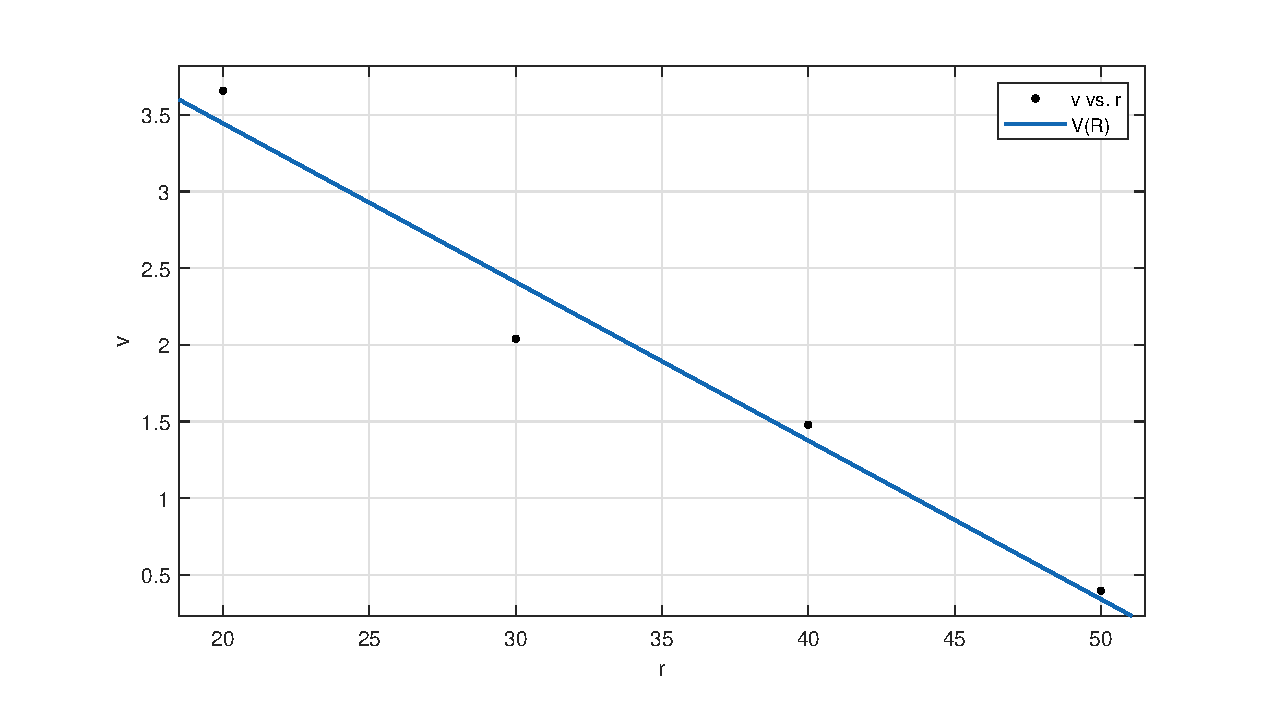
\includegraphics[width=\textwidth]{fig/KY-026/dzialanie_ukladu/charak_RV_e.eps}
    \caption{Charakterystyka zależności wrażliwości od rezystancji.}
    \label{sch}
\end{figure}

Jest to liniowość, która występuje jednak w zakresie, gdzie czujnik nie jest nadmiernie wrażliwy. W przypadku za wysokiej wrażliwości wykrycie płomienia jest mało prawdopodobne, bo np. w słoneczny dzień sensor wykrywać będzie również promienie słoneczne. 
\clearpage
\printbibliography[heading=bibintoc]

\end{document}